\chapter{Functional design} \label{chap:func_design}
\section{Background knowledge}
\subsection{Spin states}
Spin, at least in quantum mechanics, is the intrinsic angular momentum of a particle, which is described by the quantum number of the particle. Importantly, it differs from the angular momentum in classical mechanics, which is extrinsic. Spin characterizes systems of particles, usually electrons, using quantum entanglement. This phenomenon refers to the "entanglement", or spin correlation, of a set of particles.

These foundational concepts make it possible to describe quantum systems using various states. The most simple states, used as descriptors, are the energy states. Ground states refer to the system being in an energy minimum. On the other hand, excited states signify that the system has more energy than at its ground state. Additionally, there can be intermediate states during state transition.

While the aforementioned states describe system energy, they have no bearing on the spin. For the purposes of this project, only two spin states need to be explained. The first one is called singlet state. It occurs when an entangled system has a total spin of 0, caused by the mutual cancellation of spin. For example, for a system of two entangled electrons to be a singlet, the two spins would need to point in opposite directions. The second spin state is called triplet and it has a total spin of 1. Triplets can consist of, for instance, two unpaired electrons with aligned spins that sum up to 1. Singlets and triplets both have major distinguishing features and properties, which is why they can be used for quantum sensing. Aside from the difference in spin, triplets tend to have higher energy levels. They also exhibit attraction to magnetic fields, while singlets cannot be influenced directly by magnetism.

%\subsection{Energy levels and state transitions} and Zero-field splitting
\subsection{Zeeman effect}
Discovered by Pieter Zeeman in 1896, the Zeeman effect is another important phenomenon that enables quantum sensing. If under normal circumstances a light-emitting quantum system only emits one spectral line, then when a magnetic field is applied to it the line will split, thus exhibiting the Zeeman effect. In an NV center, this phenomenon causes the $\ket{\pm1}$ energy level to split into $\ket{+1}$ and $\ket{-1}$. 

\subsection{Energy levels}\label{chap:energy_levels}
Figure \ref{fig:energylevels} shows the energy level diagram of an NV center.

\begin{figure}[ht]
	\centering
	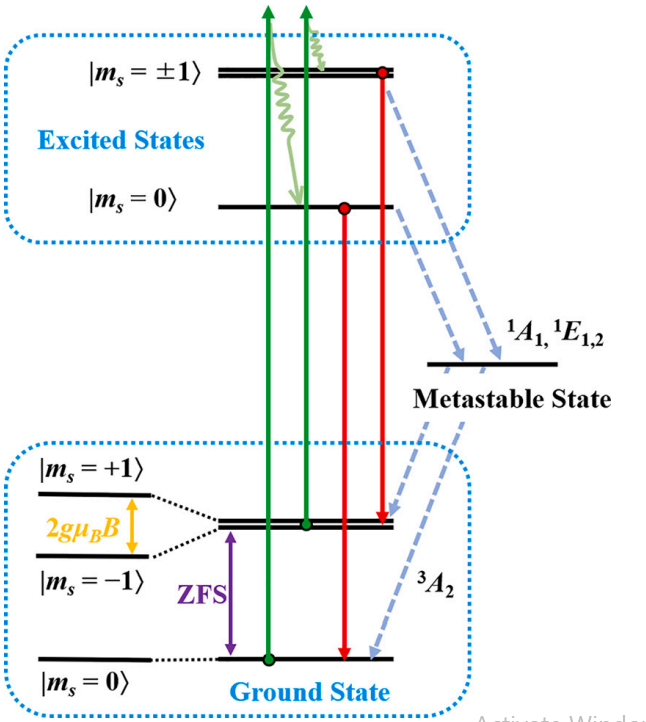
\includegraphics[width=0.7\linewidth]{img/energy_levels}
	\caption{NV center energy level diagram (image credit to Song et al \cite{song2024enhancing})}
	\label{fig:energylevels}
\end{figure}

After illuminating the NV center with a green laser, electrons go from a ground state to an excited state. They then need to return to the ground state. This decay process is usually direct and emits a red photon, however it can also go through the metastable singlet state and emit an infrared photon. It should be noted that whenever the NV center is exposed to the resonant frequency $\nu = 2,87 GHz$ the probability of emitting an infrared photon is significantly increased.


\section{Quantum protocols}
There are a number of different quantum protocols, which differ in what they can measure, in how precisely they can measure it and in the complexity of the hardware they require to operate. CW-ODMR is the main protocol this project is aimed at facilitating. As Saijo et al \cite{saijo2018ac} demonstrate, CW-ODMR is relatively simple, while still detecting magnetic field with reasonable sensitivity. Pulsed ODMR does outperform CW-ODMR \cite{zhang2020high}, but because of the added complexity working with it is a "Could have" (see Chapter \ref{project_boundaries}). Before being able to run pulsed ODMR on the setup at the lab, several protocols need to be implemented first \cite{sewani2020coherent}. $T_1$ measurements, which are one of the fundamentals of Magnetic Resonance Imaging (MRI), should be conducted first. Afterwards, Rabi oscillations need to be observed and measured in order to calibrate the setup. Without these intermediate protocols, pulsed ODMR cannot be performed.



\subsection{CW-ODMR}
CW-ODMR is a quantum protocol that has seen extensive usage in sensing setups that measure magnetic fields. Its working principle is centered around the photoluminescence of NV centers and the difference in light emission based on spin states. As already discussed in Chapter \ref{chap:energy_levels}, the NV center emits less visible light when at the resonant frequency $\nu$. Additionally, two more dips appear on the spectrum if a magnetic field is applied.Calculating the magnetic field can be done using the formula $h\nu = g_e\mu_BB_{AC}$ \footcite[In the formula, $h$ is the Planck constant, $g_e$ is the g-factor of the electron and $\mu_B$ is the Bohr magnetron. Knowing all other variables, $B_{AC}$ can easily be calculated.]{enwiki:1301371272}. Figure \ref{fig:cwodmr} shows an example of what a CW-ODMR spectrum might look like. 

\begin{figure}[ht]
	\centering
	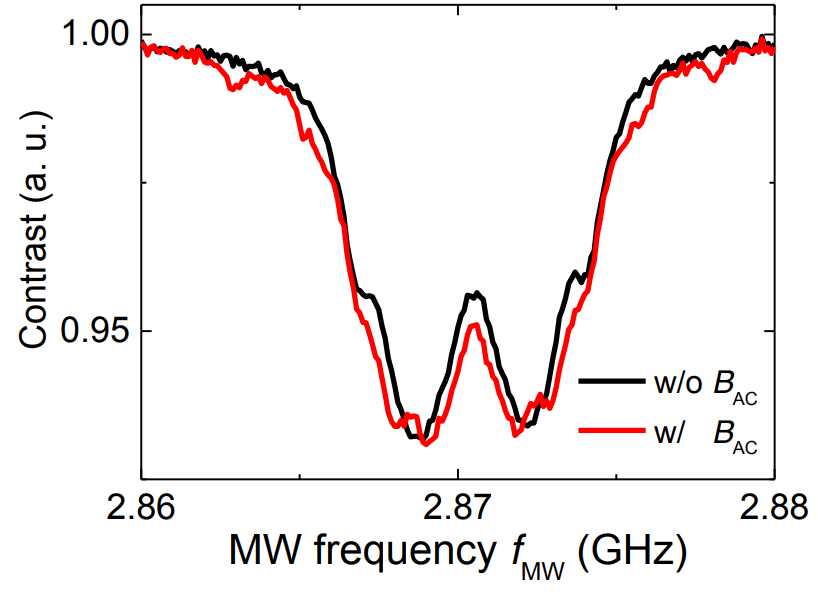
\includegraphics[width=0.7\linewidth]{img/cw_odmr}
	\caption{Spectrum of CW-ODMR \textbf{\textcolor{red}{with}} and \textbf{without} the magnetic field $B_{AC}$ (image credit Saijo et al \cite{saijo2018ac})}
	\label{fig:cwodmr}
\end{figure}


\subsection{$T_1$ relaxometry}
$T_1$, $T_2$ and $T_2^*$ relaxation time measurements are commonly associated with radiometry, but they have other uses too \cite{ballinger23}. $T_1$ measurements, in particular, are useful in the realm of quantum sensing. Knowing the $T_1$ relaxation time makes it possible to adjust the pulse sequences of more complex protocols. %explain what relaxation is and the protcol

\subsection{Pulsed ODMR}
As a more complex protocol

\section{Quantum sensing setup}
\section{Photodetection PCB}
\section{OLIA implementation}
